\chapter{A game-theoretic initialisation for the \(k\)-modes algorithm}%
\label{chp:kmodes}

\graphicspath{{chapters/kmodes/paper/img/}}
\renewcommand{\algpath}{chapters/kmodes/paper/tex/algorithms}
\renewcommand{\texpath}{chapters/kmodes/paper/tex}

\begin{center}
    The research reported in this chapter has led to a manuscript
    entitled:\\[.5em]

    {%
        \bf\itshape{``A novel initialisation based on hospital-resident
                    assignment for the \(k\)-modes algorithm''}
    }

    Submitted to: \emph{Knowledge and Information Systems}\\[.5em]

    Available online at: \arxiv{2002.02701}\\
    Associated data and source code:~\doi{10.5281/zenodo.3639282}\\[1em]

    The abstract of the manuscript is as follows:\\[.5em]
\end{center}

This paper presents a new way of selecting an initial solution for the
\(k\)-modes algorithm that allows for a notion of game theoretic fairness that
classic initialisations, namely those by Huang and Cao, do not. The method,
which utilises the Hospital-Resident Assignment Problem to find the set of
initial cluster centroids, is compared with two initialisation methods for
\(k\)-modes: the original presented in~\cite{Huang1998} and the next most
popular method present in the literature~\cite{Cao2009}. In order to highlight
the merits of the proposed method two stages of analysis are presented. The
paper concludes with an analysis of these methods against the proposed and it is
demonstrated that the proposed method is able to outperform them both. The aim
of this analysis is two-fold: first, to highlight the merits of the method in a
familiar setting by clustering well-known benchmark datasets; and second, to
provide a deeper insight into how the methods perform against one another by
generating artificial datasets using the method set out in~\cite{Wilde2020:edo}.

\myrule\

This chapter differs from the manuscript by including a more detailed
description of the \(k\)-modes algorithm and its setting (in
Section~\ref{sec:kmodes:intro}) and omits much of the discussion around matching
games (Section~\ref{sec:inits}) which has been expanded to form parts of
Appendix~\ref{app:matching}.

\section{Introduction}\label{sec:kmodes:intro}

The case study at the end of Chapter~\ref{chp:edo} examined the \(k\)-means
algorithm --- a method for clustering a set of numeric data into \(k\) parts
using Euclidean distance and the cluster means. This chapter considers another
algorithm in the \(k\)-means paradigm, \(k\)-modes, described in a set of
seminal papers by Huang~\cite{Huang1997a, Huang1997b, Huang1998}. The
\(k\)-modes algorithm makes use of similar principles to \(k\)-means, i.e.
adjusting the partition toward some Voronoi tessellation according to a measure
of centrality. However, the method allows for the clustering of categorical data
by considering a cluster's modal values rather than its mean.

The \(k\)-modes algorithm will be used to cluster patient records based on a
number of features in Chapter~\ref{chp:copd}, of which some are categorical. To
cluster data of mixed type in the \(k\)-means paradigm, the \(k\)-prototypes
algorithm may be used. The \(k\)-prototypes algorithm was introduced
in~\cite{Huang1998} with \(k\)-modes and works by separating the data into
numeric and categorical attributes before performing \(k\)-means on the numeric
data while performing \(k\)-modes on the categorical.

The focus of this chapter is on the initialisation of the \(k\)-modes algorithm
--- its initialisation is also used as the initialisation of \(k\)-prototypes.
Like \(k\)-means, there is no guarantee that any two runs of \(k\)-modes will
provide the same clusters; this is due to the stochastic nature of its
initialisation. Therefore, the performance of the algorithm is contingent upon
the quality of this initial solution~\cite{Huang1998}.

This chapter introduces a novel initialisation for the \(k\)-modes algorithm
that extends the method presented in~\cite{Huang1998}, referred to as Huang's
method. This new initialisation simulates an instance of the hospital-resident
assignment problem (HR) to incorporate mathematical fairness to the initial
solution and to eliminate the greedy component of Huang's method.

In addition to Huang's method, the literature revealed that the next most
commonly cited initialisation was presented by Cao et al. in~\cite{Cao2009}.
This initialisation (referred to as Cao's method) forms the basis of many other
initialisations where a notion of density is central. These two initialisations
form the set of established methods against which the proposed shall be
measured.

This chapter concludes with an analysis of all three initialisations and
demonstrates that the proposed method can outperform both of the established
initialisations using the traditional approach with benchmark datasets. In
addition to this, the method introduced in Chapter~\ref{chp:edo} provides a more
in-depth examination of the methods and how they perform against one another.
The first stage of this analysis serves the purpose of highlighting the merits
of each method in a familiar setting, and while the second stage bolsters these
observations, it provides a vigorous defence of the proposed method and exposes
the scenarios in which it excels. In turn, this second analysis not only allows
us to confirm the merit of the novel initialisation method as used in
Chapter~\ref{chp:copd}, but it also serves as a further case study highlighting
the importance of the paradigm described in Chapter~\ref{chp:edo}.

The chapter is structured as follows:
\begin{itemize}
    \item Section~\ref{sec:kmodes:intro} introduces the \(k\)-modes algorithm
        and its components.
    \item Section~\ref{sec:inits} provides an overview of the established
        initialisation methods before a statement of the proposed
        initialisation.
    \item Section~\ref{sec:results} presents analyses of the initialisations on
        benchmark and artificial datasets.
    \item Section~\ref{sec:kmodes:summary} concludes the chapter.
\end{itemize}


\subsection{The \(k\)-modes algorithm}\label{subsec:kmodes}

The following notation will be used throughout this chapter to describe the
objects associated with clustering a categorical dataset:

\begin{itemize}
    \item Let \(\mathcal{A} := A_1 \times \cdots \times A_m\) denote the
        \emph{attribute~space}. In this chapter, only categorical attributes are
        considered. So, for each \(j = 1, \ldots, m\), it follows that
        \(A_j := \left\{a_1^{(j)}, \ldots, a_{d_j}^{(j)}\right\}\) where
        \(d_j=|A_j|\) is the size of the \(j^{th}\) attribute.

    \item Let \(\mathcal{X} := \left\{X^{(1)}, \ldots, X^{(N)}\right\} \subset
        \mathcal{A}\) denote a \emph{dataset} where each \(X^{(i)} \in
        \mathcal{X}\) is defined as an \(m\)-tuple \(X^{(i)} := \left(x_1^{(i)},
        \ldots, x_m^{(i)}\right)\) where \(x_j^{(i)} \in A_j\) for each \(j = 1,
        \ldots, m\). The elements of \(\mathcal{X}\) are referred to as
        \emph{data points} or \emph{instances}.
    \item Let \(\mathcal{Z} := \left(Z_1, \ldots, Z_k\right)\) be a partition
        of a dataset \(\mathcal{X} \subset \mathcal A\) into \(k \in
        \mathbb{Z}^{+}\) distinct, non-empty parts. Such a partition
        \(\mathcal{Z}\) is called a \emph{clustering} of \(\mathcal{X}\).

    \item Each cluster \(Z_l\) has associated with it a
        \emph{mode} (see Definition~\ref{def:mode}) which is
        denoted by \(z^{(l)} = \left(z_1^{(l)},~\ldots,~z_m^{(l)}\right) \in
        \mathcal{A}\). These points are also referred to as
        \emph{representative~points} or \emph{centroids}. The set of all current
        cluster modes is denoted as \(\overline Z = \left\{z^{(1)}, \ldots,
        z^{(k)}\right\}\).
\end{itemize}

As discussed in Chapter~\ref{chp:lit}, the \(k\)-modes algorithm relies on a
different metric to the traditional Euclidean distance since it breaks down in a
categorical attribute space; if the space were ordinal, like the natural
numbers, then some sense of Euclidean distance could be recovered. However, in
the absence of direction or what comes between two points, this distance is not
well-defined.

There are numerous measures available for the handling of categorical data.
Definition~\ref{def:dissim} describes what is perhaps the simplest of those
measures, and is the measure used in the seminal works by
Huang~\cite{Huang1997a,Huang1997b,Huang1998}. The pitfall of this measure is
that it democratises the attribute space. In doing so, it does not fully
consider the frequency (and, thus, density) of the attributes' values, which may
result in some loss of learning by the algorithm. Examples of categorical
distance measures that do consider such properties of the attribute space
include Ng's distance~\cite{Ng2007} and, more recently, the metric introduced
in~\cite{Cao2012}.

\begin{definition}\label{def:dissim}
    Let \(\mathcal{X} \subset \mathcal A\) be a dataset and consider any
    \(X^{(a)}, X^{(b)} \in \mathcal{X}\). The dissimilarity between \(X^{(a)}\)
    and \(X^{(b)}\), denoted by \(d\left(X^{(a)}, X^{(b)}\right)\), is given by:
    \begin{equation}\label{eq:dissim}
        d\left(X^{(a)}, X^{(b)}\right) := \sum_{j=1}^{m} \delta\left(x_j^{(a)},
        x_j^{(b)}\right) \quad \text{where} \quad \delta\left(x, y\right) =
        \begin{cases}
            0, & \text{if} \ x = y \\
            1, & \text{otherwise.}
        \end{cases}
    \end{equation}

    This distance measure satisfies the properties of identity, positivity,
    symmetry and the triangle inequality, making it a metric on the attribute
    space. A proof of this can be seen as follows.

    \begin{proof}
        Let \(\mathcal A\) be a categorical attribute space. For \(d\) to be a
        metric, it must satisfy the following conditions for every \(A, B, C \in
        \mathcal A\):
        \begin{enumerate}
            \item Identity: \(d(A, B) = 0 \iff A = B\)
            \item Positivity: \(d(A, B) \geq 0\)
            \item Symmetry: \(d(A, B) = d(B, A)\)
            \item The triangle inequality: \(d(A, C) \leq d(A, B) + d(B, C)\)
        \end{enumerate}

        So, consider any \(A, B, C \in \mathcal A\).
        \begin{enumerate}
            \item Consider any \(A, B \in \mathcal A\) such that
                \(d(A, B) = 0\). Then:
                \[
                    \begin{aligned}
                        d(A, B) = 0
                        & \iff \delta\left(a_j, b_j\right) = 0 \text{, for all }
                            j=1,\ldots,m\\
                        & \iff a_j = b_j \text{, for all } j=1,\ldots,m\\
                        & \iff A = B
                    \end{aligned}
                \]
            \item If \(A = B\), then it follows from the above that
                \(d(A, B) = 0\). Otherwise, \(\delta\left(a_j, b_j\right) = 1\)
                for at least one \(j = 1, \ldots, m\). Therefore,
                \(d(A, B) \geq 1 > 0\).
            \item This follows immediately from the definition of \(\delta\)
                in~\eqref{eq:dissim}.
            \item Let \(\epsilon(A, B) = \left\{j : a_j \neq b_j\right\}\) for
                every \(A, B \in \mathcal A\), i.e. let us consider the set of
                indices where two points differ. Then it follows that
                \(d(A, B) = \abs*{\epsilon (A, B)}\). Hence:
                \[
                    \begin{aligned}
                        d(A, C) = \abs*{\epsilon(A, C)}
                        & \leq \abs*{\epsilon(A, B) \cup \epsilon(B, C)}\\
                        & \leq \abs*{\epsilon(A, B)} + \abs*{\epsilon(B, C)}\\
                        & = d(A, B) + d(B, C)
                    \end{aligned}
                \]
        \end{enumerate}

        Therefore, \(d\) satisfies the required conditions and is a metric.
    \end{proof}
\end{definition}

With the definition of a categorical distance metric, the notion of a
representative point of a cluster can be addressed. When considering numeric
data with \(k\)-means, a representative point is the mean of the points within
the cluster. With categorical data, however, the mode is used as the measure for
central tendency. This change follows from the concept of dissimilarity defined
in~\eqref{eq:dissim}. Here, the point that best represents (i.e.\ is closest to)
those in a cluster is one with the most frequent attribute values of the points
in the cluster. The following definitions formalise this notion, and
Theorem~\ref{thm:mode} provides a method to find such a point.

\begin{definition}\label{def:mode}
    Let \(\mathcal{X} \subset \mathcal{A}\) be a dataset and consider some point
    \(z = \left(z_1, \ldots, z_m\right) \in \mathcal{A}\). Then \(z\) is called
    a \emph{mode} of \(\mathcal{X}\) if it minimises the summed dissimilarity:
    \begin{equation}\label{eq:summed-dissim}
        D\left(\mathcal{X}, z\right) = \sum_{i=1}^{N} d\left(X^{(i)}, z\right)
    \end{equation}
\end{definition}

\begin{definition}\label{def:rel-freq}
    Let \(\mathcal{X} \subset \mathcal{A}\) be a dataset. Then
    \(n\left(a_s^{(j)}\right)\) denotes the \emph{frequency} of the \(s^{th}\)
    category \(a_s^{(j)}\) of \(A_j\) in \(\mathcal{X}\), i.e. for each \(A_j
    \in \mathcal{A}\) and each \(s = 1, \ldots, d_j\), it follows that:
    \begin{equation}
        n\left(a_s^{(j)}\right) := \abs*{%
            {\left\{X^{(i)} \in \mathcal{X}: x_j^{(i)} = a_s^{(j)}\right\}}
        }
    \end{equation}

    Furthermore, \(\frac{n\left(a_s^{(j)}\right)}{N}\) is called the
    \emph{relative~frequency} of category \(a_s^{(j)}\) in \(\mathcal{X}\).
\end{definition}

\begin{theorem}\label{thm:mode}
    Consider a dataset \(\mathcal{X} \subset \mathcal{A}\) and some \(U = (u_1,
    \ldots, u_m) \in \mathcal{A}\). Then \(D(\mathcal{X}, U)\) is minimised if
    and only if \(n\left(u_j\right) \geq n\left(a_s^{(j)}\right)\) for all
    \(s=1, \ldots, d_j\) and each \(j = 1, \ldots, m\).

    A proof of this theorem can be found in the Appendix of~\cite{Huang1998}.
\end{theorem}

Theorem~\ref{thm:mode} defines the process by which cluster modes are updated in
\(k\)-modes --- specifically, in Algorithm~\ref{alg:update}. Therefore, the
final component from the \(k\)-means paradigm to be configured is the objective
(cost) function. This function is defined in Definition~\ref{def:cost}, and
following that a practical statement of the \(k\)-modes algorithm is given in
Algorithm~\ref{alg:kmodes} as set out in~\cite{Huang1998}.

\begin{definition}\label{def:cost}
    Let \(\mathcal{Z} = \left\{Z_1, \ldots, Z_k\right\}\) be a clustering of a
    dataset \(\mathcal{X}\), and let \(\overline Z = \left\{z^{(1)},
    \ldots, z^{(k)}\right\}\) be the corresponding cluster modes. Then \(W =
    \left(w_{i, l}\right)\) is an \(N \times k\) \emph{partition~matrix} of
    \(\mathcal{X}\) such that:
    \[
        w_{i, l} = \begin{cases}
                     1, & \text{if} \ X^{(i)} \in Z_l\\
                     0, & \text{otherwise.}
                   \end{cases}
    \]

    With this, the \emph{cost~function} is defined to be the summed
    within-cluster dissimilarity:
    \begin{equation}\label{eq:cost}
        C\left(W, \overline Z\right) := \sum_{l=1}^{k} \sum_{i=1}^{N}
        \sum_{j=1}^{m} w_{i,l} \ \delta\left(x_j^{(i)}, z_j^{(l)}\right)
    \end{equation}
\end{definition}

\inputalg{kmodes}


\section{Initialisation processes}\label{sec:inits}

The \(k\)-modes algorithm is stochastic, in that it is dependent on a stochastic
choice of starting point. The process of finding an initial solution or set of
modes for the algorithm is called the initialisation. As with many algorithms in
the centroid-based paradigm, the standard initialisation for \(k\)-modes is to
randomly sample \(k\) distinct points in the dataset, call them the initial
modes and assign each data point to its closest mode.

The initial set of modes must be instances in the dataset to ensure that there
are no empty clusters in the first iteration of the algorithm. However, this set
of points need not be determined entirely at random. The remainder of this
section describes two well-established initialisations for \(k\)-modes that aim
to lever the structure of the data at hand preemptively to select these initial
modes. The section then closes with the motivation and definition of the
proposed initialisation method.

\subsection{Huang's method}\label{subsec:huang}

Among the original works by Huang, an alternative initialisation method was
presented that selects modes by distributing frequently occurring values from
the attribute space among \(k\) potential modes~\cite{Huang1998}. The process
(referred to as Huang's method) is described in full in
Algorithm~\ref{alg:huang}. Huang's method considers a set of potential modes,
\(\widehat Z \subset \mathcal A\), that is then replaced by a set of real
initial modes, \(\overline Z \subset \mathcal X\).

The process of selecting this set of potential modes is ambiguous in the
original paper --- as is alluded to in~\cite{Jiang2016}. In~\cite{Huang1998},
the author states that the potential modes should be created by assigning to
them the ``most frequent categories equally''. Here, as is done in practical
implementations of \(k\)-modes, this assignment is interpreted as a weighted
random sample. Algorithm~\ref{alg:potential_modes} contains a description of the
sampling process using the relative frequencies of the values (categories) in
the attribute space.

\inputalg{huang}


\subsection{Cao's method}\label{subsec:cao}

The second initialisation considered in this chapter is known as Cao's
method~\cite{Cao2009}. This method differs significantly from Huang's method,
and has formed the basis of several other initialisations. In essence, the
method selects initial modes according to their density in the dataset whilst
forcing dissimilarity between them. Definition~\ref{def:density} formalises the
concept of categorical density. The definition also considers the relationship
between density and relative frequency when using the measure defined
in~\eqref{eq:dissim}.

Further to its alternative density-based approach, the method (which is
described in Algorithm~\ref{alg:cao}) is deterministic. Therefore, when using
\(k\)-modes with Cao's initialisation, only one run of the algorithm is required
to identify a clustering, making it an attractive option if computational time
is critical.

\begin{definition}\label{def:density}
    Consider a dataset \(\mathcal{X} \subset \mathcal{A} = \{A_1,\ldots,A_m\}\).
    Then~\cite{Cao2009} defines the \emph{average~density} of any point
    \(X^{(i)} \in \mathcal{X}\) with respect to \(\mathcal{A}\) as:
    \begin{equation}\label{eq:density}
        \text{Dens}\left(X^{(i)}\right) 
        = \frac{\sum_{j=1}^m \text{Dens}_{j}\left(X^{(i)}\right)}{m}
    \end{equation}

    \noindent where
    \begin{equation}
        \text{Dens}_{j}\left(X^{(i)}\right) 
        = \frac{%
            \abs*{%
                \left\{X^{(t)} \in \mathcal{X} : x_j^{(i)} = x_j^{(t)}\right\}
            }
        }{N}
        = \frac{n \left(x_j^{(i)}\right)}{N}
    \end{equation}

    That is, \(\text{Dens}_j \left(X^{(i)}\right)\) is the relative
    frequency of \(x_j^{(i)}\) in \(\mathcal X\). Also, observe that:
    \begin{equation}
        \abs*{\left\{X^{(t)} \in \mathcal{X} : x_j^{(i)} = x_j^{(t)}\right\}}%
        = \sum_{t=1}^N \left(1 - \delta\left(x_j^{(i)}, x_j^{(t)}\right)\right)
    \end{equation}

    Hence, an alternative definition for~\eqref{eq:density} can be derived:
    \begin{equation}\label{eq:density-alt}
        \text{Dens}\left(X^{(i)}\right)
        = \frac{1}{mN} \sum_{j=1}^m \sum_{t=1}^N \left(%
            1 - \delta\left(x_j^{(i)}, x_j^{(t)}\right)
        \right)
        = 1 - \frac{1}{mN} D\left(\mathcal{X}, X^{(i)}\right)
    \end{equation}

    This alternative definition highlights how identifying high-density data
    points would mean finding data points with a low summed dissimilarity, i.e.
    true modes of the dataset.
\end{definition}

\inputalg{cao}


\subsection{The proposed method}\label{subsec:method}

Both of the initialisation methods described in this section have a greedy
component. Cao's method essentially chooses the point with highest density that
has not already been chosen whilst forcing some separation between the set of
initial modes. In the case of Huang's, the greediness only comes toward the end
of the method. When the set of potential modes is identified, it is replaced by
a set of instances in the dataset. Specifically, this means that in any
practical implementation of this method, the order in which a set of potential
modes is iterated over can affect the set of initial modes. Thus, there is no
guarantee of consistency. The same is true for any arbitrary tie breaks that may
occur.

The initialisation proposed in this chapter extends Huang's method to be
order-invariant in the final allocation. Doing so eliminates its greedy
component and provides a more intuitive starting point for the \(k\)-modes
algorithm by constructing and solving a matching game between the set of
potential modes and some subset of the data.

Matching games are a construct from game theory that allow for the allocation of
partnerships between agents (players) such that no pair of players is rationally
envious of any partnership. Appendix~\ref{app:matching} provides an extensive
introduction to several fundamental matching games, the most commonly found of
which is the stable marriage problem (SM). SM, like many matching games,
involves two distinct sets of players (parties), each of whom have a strict
ranking of the players in the other set. Resolving these player preferences to
find a matching in which no two players would rather be matched to one another
than their current matches is called \emph{solving} the game. The authors
of~\cite{Gale1962} formalised this problem and provided an algorithm that
guarantees to find an stable, party-optimal matching to any instance of SM. This
algorithm is given in Appendix~\ref{app:matching}, and algorithms following a
similar structure are commonly referred to as Gale-Shapley algorithms.

Despite its simplicity, using SM in this scenario would reduce the proposed
method to Huang's method. This can be seen as follows. Both parties in the game
must be of the same size, and so \(k\) data points must be considered along with
the potential modes. The most straightforward way of selecting these points is
to allow each potential mode to add its closest point that has not already been
selected. Then, upon solving the game, and up to an arbitrary breaking of any
ties in the preference lists, each potential mode is assigned to its chosen data
point.

A popular generalisation of SM is HR, a matching game that addresses the
practical problem from which it gets its name: assigning medical students to
hospital placements. A variant of this game is still used by the National
Resident Matching Program (NRMP) in the United States. A thorough description of
HR, and the algorithms to solve instances of it, is provided in
Appendix~\ref{app:matching}. However, a brief overview is provided here.

Consider two distinct sets of players, \(R\) and \(H\), and call them the
residents and hospitals, respectively. In HR, every resident \(r \in R\)
provides a strict ranking of some nonempty subset of the hospitals, denoted
\(f(r)\). Then, each hospital \(h \in H\) provides a preference list, \(g(h)\),
strictly ranking all and only those residents that have ranked it, i.e. \(g(h)\)
is some permutation of the set \(\left\{r \in R \ | \ h \in f(r)\right\}\). In
addition to these preference lists, HR stipulates that every hospital \(h \in
H\) has a capacity, \(c_h \in \mathbb N\), associated with them. This capacity
is a strict upper limit on the number of residents that a hospital may be
matched to at once. A general assumption, although not necessary, is that there
is sufficient capacity across the hospitals for all of the residents to be
assigned, i.e. that \(\sum_{h \in H} c_h \ge \lvert R \rvert\). This
construction of residents, hospitals, preference lists and capacities form a
\emph{game}, denoted by \((R, H)\).

The objective of the game is to identify a many-to-one mapping (referred to as a
\emph{matching}), \(M\), between the residents and the hospitals. In particular,
the aim is to find a matching such that no resident-hospital pair could be, and
would rather be, matched to one another than their current match(es). Such a
matching is considered \emph{stable}. Finding a resident- or hospital-optimal,
stable matching to an instance of HR is called \emph{solving} the game. In
addition to SM, the authors formalised HR in~\cite{Gale1962}, and presented a
Gale-Shapley algorithm that guaranteed such a solution to any instance of the
game. Subsequent studies~\cite{Dubins1981,Roth1984} have improved on the
original algorithm by leveraging structures within the game, such as the strict
nature of the preference lists.

Returning to the problem at hand, where the \(k\) potential modes must
be allocated to a nearby and unique data point, it can be seen that HR mirrors
the constraints well. In particular, this scenario can be modelled by an
instance of HR where each hospital has a capacity of one. A contextual summary
of the remaining HR game components and those of the proposed initialisation is
given in Table~\ref{tab:components}.

\begin{table}[htbp]
    \resizebox{\textwidth}{!}{%
    \begin{tabular}{lcr}
        \toprule%
        Object in \(k\)-modes initialisation & {} & Object in a matching game
        \\\midrule%
        Potential modes & {} & The set of residents
        \\
        Data points closest to potential modes & {} & The set of hospitals
        \\
        Similarity between a potential mode and a point & {} & Position in 
        preference lists
        \\
        The data point to replace a potential mode & {} & A pair in a matching
        \\\bottomrule
    \end{tabular}}
    \caption{%
        Links between the initialisation and the components of a game
    }\label{tab:components}
\end{table}

A limitation of using HR is the common occurrence of ties when using the
distance measure defined in~\eqref{eq:dissim}. A tie in the distance between
points corresponds to a tie in the preference lists. As is discussed in
Appendix~\ref{app:matching}, extensions to HR do exist for handling ties in
preferences that would alleviate the reliance on having to break ties. However,
the notion of stability becomes tiered under such extensions, and the guarantee
of a stable matching does not exist. Therefore, they are not considered here.
Instead, the proposed method employs the standard form of HR and aims to
mitigate the effect of ties by considering a potentially large number of
candidate points (up to \(k^2\)). Algorithm~\ref{alg:proposed_method} provides a
formal statement of the proposed method.

\inputalg{proposed_method}


\section{Experimental results}\label{sec:results}

This section provides several analyses of the initialisation processes presented
in this chapter. Each analysis herein requires the use of software, and
specifically an implementation of the \(k\)-modes algorithm. The implementation
used, called \mintinline{console}{kmodes}, is available on the Python Package
Index and its source code is hosted on GitHub~\cite{deVos2015}. Huang's and
Cao's methods are implemented already in \mintinline{console}{kmodes}, and the
proposed matching initialisation has been included in a separate fork of the
GitHub repository, available at~\doi{10.5281/zenodo.3713170}. This version of
the \(k\)-modes implementation makes use of a Python library, \matching, the
details of which can be found in Appendix~\ref{app:matching}. The version of the
library used for these analyses is available at~\doi{10.5281/zenodo.2711847}.
Furthermore, all of the source code used in this section is available
at~\doi{10.5281/zenodo.3639282}.

To give comparative results on the quality of the initialisation processes
considered in this chapter, four well-known, categorical, labelled datasets ---
breast cancer, mushroom, nursery, and soybean (large) --- will be clustered by
the \(k\)-modes algorithm with each of the initialisation processes. These
datasets have been chosen to fall in line with the established literature, and
particularly the works in which Huang's and Cao's methods were introduced.
Further, the datasets exhibit a range of sizes, complexities and applications.
Each dataset is openly available under the University of California Irvine (UCI)
Machine Learning Repository~\cite{Dua2019}, and their characteristics are
summarised in Table~\ref{tab:dataset_summary}. This analysis excludes all
incomplete instances (i.e.\ where data is missing), and the remaining dataset
characteristics are reported as `adjusted'.

\begin{table}
    \resizebox{\textwidth}{!}{\input{\texpath/dataset_summary}}
    \caption{A summary of the benchmark datasets}\label{tab:dataset_summary}
\end{table}

This analysis does not consider evaluative metrics related to classification
such as accuracy, recall or precision --- although this is commonly done. A
selection of articles from the last 20 or so years that employ this approach
include~\cite{%
    Arthur2007,Cao2009,Cao2012,Huang1998,%
    Ng2007,Olaode2014,Schaeffer2007,Sharma2015%
}. Instead, only internal measures are considered, such as the cost function
defined in~\eqref{eq:cost}. Like inertia with \(k\)-means, this metric is
label-invariant, and its values are comparable across the different
initialisation methods on the same dataset. Furthermore, the cost function
captures the effect of each initialisation method on the initial and final
clustering of each dataset.

An additional, and often useful, metric for clustering is the silhouette
coefficient. In Chapter~\ref{chp:edo}, the silhouette served as an extension to
the cost function to ensure intra-cluster cohesion and inter-cluster separation.
Therefore, it would be sensible to believe that it could provide insight into
the effect of each initialisation method to the \(k\)-modes algorithm. However,
this metric loses its intuition under the distance measure employed here. As
such, it has been omitted. The remaining performance measures used are the
number of iterations for the \(k\)-modes algorithm to terminate after the
initialisation and the time to terminate in seconds.

The final piece of information required in this analysis is a choice for \(k\)
for each dataset. An immediate choice is the number of classes that are present
in a dataset, but this is not necessarily an appropriate choice since the
classes may not be representative of true clusters~\cite{Memoli2011}. However,
this analysis will consider this case as there may be practical reasons to limit
the value of \(k\). The other strategy for choosing \(k\) considered in this
chapter uses the knee point detection algorithm introduced
in~\cite{Satopaa2011}. This strategy was chosen over other popular methods such
as the `elbow' method as its results are definitive.

The knee point detection algorithm was employed using values of \(k\) from 2 up
to \(\lfloor\sqrt N\rfloor\) for each dataset. The number of clusters determined
by this strategy is reported in the final column of
Table~\ref{tab:dataset_summary}.


\subsection{Using the knee point detection algorithm for \(k\)}
\label{subsec:knee}

Table~\ref{tab:metrics_knee} summarises the results of each initialisation
method on the benchmark datasets. In each case, the number of clusters was
determined using the knee point detection algorithm. Each column shows the mean
value of each metric and its standard deviation across
\input{chapters/kmodes/paper/tex/repetitions.tex}repetitions of the \(k\)-modes
algorithm.

\begin{table}
    \begin{subtable}{\textwidth}
        \resizebox{\textwidth}{!}{%
            \input{\texpath/knee/breast_cancer_summary.tex}
        }
        \caption{%
            the breast cancer dataset with \(k=8\)%
        }\label{tab:breast_cancer_knee}
    \end{subtable}\vspace{1em}

    \begin{subtable}{\textwidth}
        \resizebox{\textwidth}{!}{\input{\texpath/knee/mushroom_summary.tex}}
        \caption{%
            the mushroom dataset with \(k=17\)%
        }\label{tab:mushroom_knee}
    \end{subtable}\vspace{1em}

    \begin{subtable}{\textwidth}
        \resizebox{\textwidth}{!}{\input{\texpath/knee/nursery_summary.tex}}
        \caption{%
            the nursery dataset with \(k=23\)
        }\label{tab:nursery_knee}
    \end{subtable}\vspace{1em}

    \begin{subtable}{\textwidth}
        \resizebox{\textwidth}{!}{\input{\texpath/knee/soybean_summary.tex}}
        \caption{%
            the soybean dataset with \(k=8\)
        }\label{tab:soybean_knee}
    \end{subtable}

    \caption{%
        Metric results when using the knee point detection algorithm
    }\label{tab:metrics_knee}
\end{table}

By examining these tables, it would seem that the proposed method and Huang's
method are fairly comparable across the board. On the contrary, the proposed
method is faster despite taking more iterations in general which suggests a more
intuitive initialisation. More importantly, though, it appears that Cao's method
performs the best out of the three initialisation methods. In terms of initial
and final costs Cao's method improves by roughly 10\% against the next best
method for the three datasets with which it succeeds. Also, while the number of
iterations is comparable, the computation time is substantially less than the
other two methods. This last observation is expected given it is a deterministic
method and need only be run once to achieve this performance.

As useful as these metrics are, in the centroid-based clustering paradigm, a
particular clustering is selected based on it having the minimal final cost over
several runs of the algorithm --- not the mean. While Cao's method is reliable
in this regard, in that there is no variation at all, it does not always produce
the best clustering possible. There is a trade-off to be made between
computational time and performance here.

In order to gain more insight into the performance of each method, a less
granular form of analysis is required.
Figures~\ref{fig:breast_cancer_knee}---\ref{fig:soybean_knee} display the cost
function results for each dataset in the form of a scatter plot and two
empirical cumulative density function (CDF) plots, highlighting the breadth and
depth of the behaviours exhibited by each initialisation method.

Looking at Figure~\ref{fig:breast_cancer_knee}, it is clear that in terms of the
final cost, Cao's method is middling when compared to the other methods. This
so-so performance is apparent from Table~\ref{tab:breast_cancer_knee} and,
indeed, Huang's and the proposed method appear indistinguishable when looking at
the body of the results. However, since the criterion for the best clustering
(in practical terms) is having the minimal final cost, the proposed method is
superior; that the method produces clusterings with a broader range of costs
(indicated by the trailing right-hand side of each CDF plot) is irrelevant for
the same reason.

This pattern of broadly similar behaviour between Huang's and the proposed
method is apparent in each of the figures here, and in all cases, the proposed
method outperforms Huang's. In fact, for all cases except for the nursery
dataset, the proposed method achieves the lowest final cost of all the methods.
As such, it performs the best in practical terms on these particular datasets.

In the case of the nursery dataset, Cao's method is unquestionably the best
performing initialisation method. There are two things of note here: first, not
one of the methods was able to find an initial clustering that \(k\)-modes could
improve upon; and, second, the nursery dataset exactly describes the entire
attribute space in which it exists. This property could be why the other methods
fall behind Cao's method so decisively. In such a scenario, Cao's method can
definitively choose the \(k\) most dense-whilst-separated points from that
space as the initial cluster centres. Meanwhile, the two remaining methods are,
in essence, randomly sampling from this space. That each initial solution in
these repetitions is locally optimal remains a mystery.

\begin{figure}
    \begin{subfigure}{.5\textwidth}
        \includegraphics[width=\linewidth]{Fig1a.pdf}
        \caption{Scatter plot of initial and final costs.}
    \end{subfigure}
    \hfill%
    \begin{subfigure}{.5\textwidth}
        \includegraphics[width=\linewidth]{Fig1b1.pdf}

        \includegraphics[width=\linewidth]{Fig1b2.pdf}
        \caption{Empirical CDF plots for initial (top) and final (bottom)
                 costs.}
    \end{subfigure}
    \caption{Summary plots for the breast cancer dataset with \(k=8\)}%
    \label{fig:breast_cancer_knee}
\end{figure}

\begin{figure}
    \begin{subfigure}{.5\textwidth}
        \includegraphics[width=\linewidth]{Fig2a.pdf}
        \caption{Scatter plot of initial and final costs.}
    \end{subfigure}
    \hfill%
    \begin{subfigure}{.5\textwidth}
        \includegraphics[width=\linewidth]{Fig2b1.pdf}

        \includegraphics[width=\linewidth]{Fig2b2.pdf}
        \caption{Empirical CDF plots for initial (top) and final (bottom)
                 costs.}
    \end{subfigure}
    \caption{Summary plots for the mushroom dataset with \(k=17\)}%
    \label{fig:mushroom_knee}
\end{figure}

\begin{figure}
    \begin{subfigure}{.5\textwidth}
        \includegraphics[width=\linewidth]{Fig3a.pdf}
        \caption{Scatter plot of initial and final costs}
    \end{subfigure}
    \hfill%
    \begin{subfigure}{.5\textwidth}
        \includegraphics[width=\linewidth]{Fig3b1.pdf}

        \includegraphics[width=\linewidth]{Fig3b2.pdf}
        \caption{Empirical CDF plots for initial (top) and final (bottom) costs}
    \end{subfigure}
    \caption{Summary plots for the nursery dataset with \(k=23\)}%
    \label{fig:nursery_knee}
\end{figure}

\begin{figure}
    \begin{subfigure}{.5\textwidth}
        \includegraphics[width=\linewidth]{Fig4a.pdf}
        \caption{Scatter plot of initial and final costs}
    \end{subfigure}
    \hfill%
    \begin{subfigure}{.5\textwidth}
        \includegraphics[width=\linewidth]{Fig4b1.pdf}

        \includegraphics[width=\linewidth]{Fig4b2.pdf}
        \caption{Empirical CDF plots for initial (top) and final (bottom) costs}
    \end{subfigure}
    \caption{Summary plots for the soybean dataset with \(k=8\)}%
    \label{fig:soybean_knee}
\end{figure}


\subsection{Using the number of classes for \(k\)}
\label{subsec:nclasses}

As is discussed above, the often automatic choice for \(k\) is the number of
classes present in the data. This subsection repeats the analysis from the
previous subsection but with this traditional choice for \(k\).
Table~\ref{tab:metrics_nclasses} contains the analogous summaries of each
initialisation method's performance on the benchmark datasets over the same
number of repetitions.

\begin{table}
    \begin{subtable}{\textwidth}
        \resizebox{\textwidth}{!}{%
            \input{\texpath/nclasses/breast_cancer_summary.tex}
        }
        \caption{%
            the breast cancer dataset with \(k=2\)%
        }\label{tab:breast_cancer_nclasses}
    \end{subtable}\vspace{1em}

    \begin{subtable}{\textwidth}
        \resizebox{\textwidth}{!}{%
            \input{\texpath/nclasses/mushroom_summary.tex}
        }
        \caption{%
            the mushroom dataset with \(k=2\)%
        }\label{tab:mushroom_nclasses}
    \end{subtable}\vspace{1em}

    \begin{subtable}{\textwidth}
        \resizebox{\textwidth}{!}{\input{\texpath/nclasses/nursery_summary.tex}}
        \caption{%
            the nursery dataset with \(k=5\)
        }\label{tab:nursery_nclasses}
    \end{subtable}\vspace{1em}

    \begin{subtable}{\textwidth}
        \resizebox{\textwidth}{!}{\input{\texpath/nclasses/soybean_summary.tex}}
        \caption{%
            the soybean dataset with \(k=15\)
        }\label{tab:soybean_nclasses}
    \end{subtable}

    \caption{%
        Metric results when using the number of classes
    }\label{tab:metrics_nclasses}
\end{table}

An immediate comparison to the previous tables is that the mean costs are
significantly higher, and the computation times are shorter, for all datasets
bar the soybean dataset. These effects come directly from the choice of \(k\) in
that higher values of \(k\) will require more checks (and thus computational
time) but will typically lead to more homogeneous clusters, reducing their
within-cluster dissimilarity and therefore cost.

Looking at these tables on their own reveals that Cao's method is the superior
initialisation method on average: the means are substantially lower in terms of
initial and final cost; there is no deviation in these results; again, the total
computational time is a fraction of the other two methods. It is apparent again
that Huang's and the proposed method are comparable on average. Then, as before,
a more nuanced investigation will require finer visualisations.
Figures~\ref{fig:breast_cancer_nclasses}---\ref{fig:soybean_nclasses} show the
analogous plots as in the previous subsection except with this traditional
choice for \(k\).

Figures~\ref{fig:breast_cancer_nclasses}~and~\ref{fig:mushroom_nclasses}
indicate that a particular behaviour emerged during the runs of the \(k\)-modes
algorithm. Specifically, each solution falls into one of (predominantly) two
types: effectively no improvement on the initial clustering, or terminating at
some clustering with a cost that is bounded below across all such solutions.
Invariably, Cao's method achieves this lower bound, and unless Cao's method is
used, these particular choices for \(k\) mean that the performance of the
\(k\)-modes algorithm is highly susceptible to its initial clustering. Moreover,
the other two methods are effectively indistinguishable in these cases, and so
if a robust solution is required, Cao's method is the only viable option.

Figure~\ref{fig:nursery_nclasses} corresponds to the nursery dataset results
with \(k=5\). In this set of runs, the same pattern emerges as in
Figure~\ref{fig:nursery_knee} where sampling the initial centres from amongst
the densest points (via Huang's method and the proposed) is an inferior strategy
to one considering the entire attribute space such as with Cao's method. Again,
no method can improve on the initial solution (except for one repetition with
the matching initialisation method) although the disparity between Cao's method
and the others is significantly less.

\begin{figure}
    \begin{subfigure}{.5\textwidth}
        \includegraphics[width=\linewidth]{Fig5a.pdf}
        \caption{Scatter plot of initial and final costs.}
    \end{subfigure}
    \hfill%
    \begin{subfigure}{.5\textwidth}
        \includegraphics[width=\linewidth]{Fig5b1.pdf}

        \includegraphics[width=\linewidth]{Fig5b2.pdf}
        \caption{Empirical CDF plots for initial (top) and final (bottom) costs}
    \end{subfigure}
    \caption{Summary plots for the breast cancer dataset with \(k=2\)}%
    \label{fig:breast_cancer_nclasses}
\end{figure}

\begin{figure}
    \begin{subfigure}{.5\textwidth}
        \includegraphics[width=\linewidth]{Fig6a.pdf}
        \caption{Scatter plot of initial and final costs}
    \end{subfigure}
    \hfill%
    \begin{subfigure}{.5\textwidth}
        \includegraphics[width=\linewidth]{Fig6b1.pdf}

        \includegraphics[width=\linewidth]{Fig6b2.pdf}
        \caption{Empirical CDF plots for initial (top) and final (bottom) costs}
    \end{subfigure}
    \caption{Summary plots for the mushroom dataset with \(k=2\)}%
    \label{fig:mushroom_nclasses}
\end{figure}

\begin{figure}
    \begin{subfigure}{.5\textwidth}
        \includegraphics[width=\linewidth]{Fig7a.pdf}
        \caption{Scatter plot of initial and final costs}
    \end{subfigure}
    \hfill%
    \begin{subfigure}{.5\textwidth}
        \includegraphics[width=\linewidth]{Fig7b1.pdf}

        \includegraphics[width=\linewidth]{Fig7b2.pdf}
        \caption{Empirical CDF plots for initial (top) and final (bottom) costs}
    \end{subfigure}
    \caption{Summary plots for the nursery dataset with \(k=5\)}%
    \label{fig:nursery_nclasses}
\end{figure}

\begin{figure}
    \begin{subfigure}{.5\textwidth}
        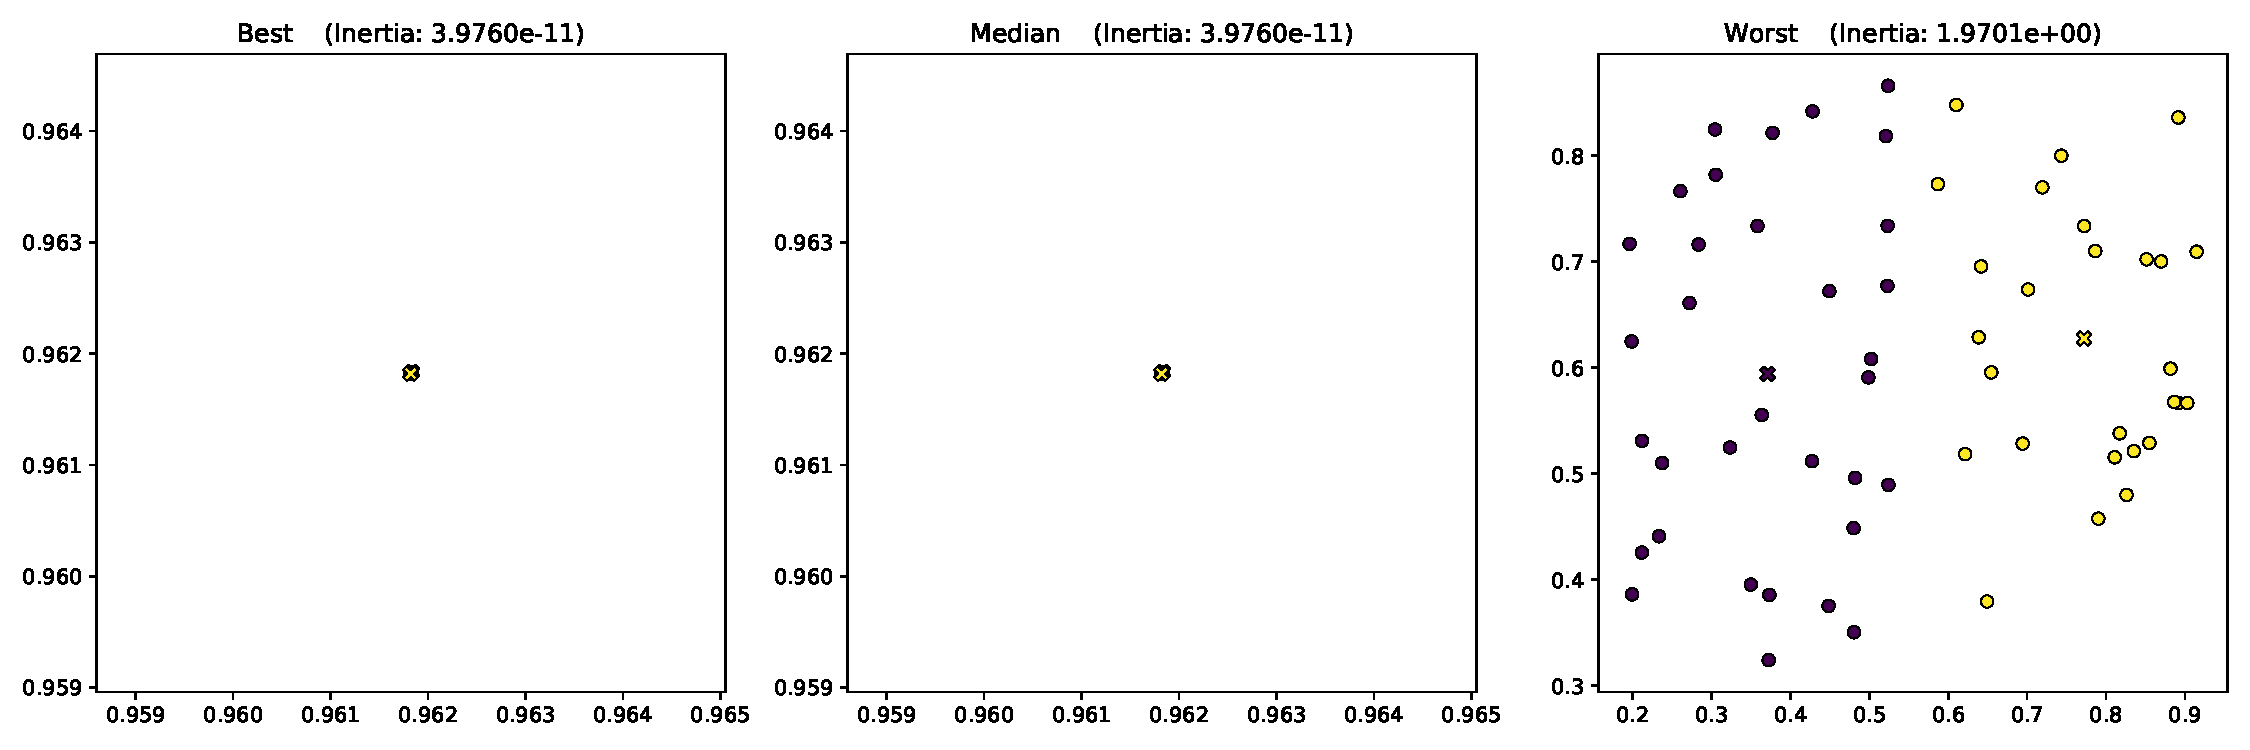
\includegraphics[width=\linewidth]{Fig8a.pdf}
        \caption{Scatter plot of initial and final costs}
    \end{subfigure}
    \hfill%
    \begin{subfigure}{.5\textwidth}
        \includegraphics[width=\linewidth]{Fig8b1.pdf}

        \includegraphics[width=\linewidth]{Fig8b2.pdf}
        \caption{Empirical CDF plots for initial (top) and final (bottom) costs}
    \end{subfigure}
    \caption{Summary plots for the soybean dataset with \(k=15\)}%
    \label{fig:soybean_nclasses}
\end{figure}

The primary conclusion from this analysis of benchmark datasets is that while
Huang's method is mostly comparable to the proposed extension, there is no
substantial evidence to use Huang's method over the one proposed in this
chapter. Figure~\ref{fig:soybean_nclasses} shows the only instance where Huang's
method was able to outperform the proposed method. Other than this, the proposed
method consistently performs better (or as well as) Huang's method in terms of
minimal final costs and computational time. This success occurs when an external
framework is imposed on the data (by choosing \(k\) to be the number of classes)
and not. Furthermore, though not discussed here, the matching initialisation
method has the scope to allow for expert or prior knowledge to be included in an
initial clustering by using some expedient or specific preference list
mechanism.

\subsection{Artificial datasets}\label{subsec:artificial}

All of the results leading up to this point were created using benchmark
datasets. The discussion at the start of Chapter~\ref{chp:edo} does not condemn
this entirely as there are certainly benefits to comparing methods in this way
such as familiarity and direct comparison. However, as elaborated on in that
discussion, it does not afford a rich understanding of how any of the methods
perform more generally. This stage of the analysis relies on the method for
generating artificial datasets introduced in Chapter~\ref{chp:edo}, and, as was
made clear in that chapter's case study, the critical component of this method
is a well-defined fitness function.

In order to expose the nuances in the performance of Cao's method and the
proposed initialisation on a particular dataset, two cases are considered: where
Cao's method outperforms that proposed, and vice versa. Both cases use the same
fitness function, although the latter uses its negative. The function is defined
as follows:

\begin{equation}\label{eq:fitness}
    f\left(\mathcal X\right) = C_{\mathrm{cao}} - C_{\mathrm{match}}
\end{equation}

Here, \(C_{\mathrm{cao}}\) and \(C_{\mathrm{match}}\) are the final costs when a
dataset \(\mathcal X\) is clustered using Cao's method and the proposed matching
method respectively with \(k = 3\). Given that costs should be minimised, this
function is given to EDO to be minimised. As such, the case that uses \(f\) will
be referred to as Cao-preferable and \(-f\) will be referred to as
matching-preferable. For the sake of computational time, the proposed
initialisation is given 25 repetitions.

Apart from the sign of \(f\), each case uses identical EDO parameters: a
population size of \(N = 500\); row and column limits of \(R = (50, 500)\) and
\(C = (2, 50)\), respectively; selection parameters \(b = 0.2\) and \(l = 0\); a
mutation probability of \(p_m = 0.01\); a maximum number of iterations of \(M =
100\). In addition to these parameters, the only distribution family included is
a discrete uniform family with up to ten categories. This means that all columns
in the generated datasets will have at least one category but no more than ten.

\begin{figure}
    \centering
    \includegraphics[width=\imgwidth]{Fig9.pdf}
    \caption{%
        Histograms of fitness for the top performing percentile in each case
    }\label{fig:fitness}
\end{figure}

This process yielded approximately 35,000 unique datasets for each case, and the
subsequent analysis only considers the top-performing percentile of datasets
from each. The datasets are available online at~\doi{10.5281/zenodo.3638035}.
Figure~\ref{fig:fitness} shows the fitness distribution of the top
percentile in each case. It should be clear from~\eqref{eq:fitness} that large
negative values are preferable here. With that, and bearing in mind that the
generation of these datasets was parameterised consistently, it appears that the
attempt to outperform Cao's method proved somewhat more straightforward than
the reverse situation; this is indicated by the substantial difference in the
locations of the fitness distributions.

Given the quantity of data available, to understand the patterns that have
emerged, they must be summarised --- as in Chapter~\ref{chp:edo}. In this case,
univariate statistics are used. Despite the datasets all being of similar
shapes, there are some discrepancies. With the number of rows, this is less of
an issue, but any comparison of statistics across datasets of different widths
is difficult without prior knowledge of the datasets. Moreover, there is no
guarantee of contingency amongst the attributes, and the comparison of more than
a handful of variables becomes complicated even when the attributes are
identifiable. To combat this and bring uniformity to the datasets, each dataset
is represented as their first principal component obtained via centred Principal
Component Analysis (PCA)~\cite{Jolliffe1986}. While some subtleties may be lost,
this representation captures the essential characteristics of each dataset in a
single variable, meaning they can be compared directly.

Since the transformation by PCA is centred, all measures for central tendency
are moot. The mean and median are not interpretable here anyway, given that the
original data is categorical. As such, the univariate statistics used here
describe the spread and shape of the principal components and are split into
two groups: central moments (variance, skewness and kurtosis) and empirical
quantiles (the interquartile range, and lower and upper deciles).

Figures~\ref{fig:edo_moments}~and~\ref{fig:edo_quantiles} show the distributions
of the six univariate statistics across all of the principal components in each
case. In addition to this, they show a fitted Gaussian kernel density
estimate~\cite{Bashtannyk2001} to accentuate the general shape of the
histograms. What is immediately clear from each of these plots is that for
datasets where Cao's method performs better, the general spread of their first
principal component is much tighter than in the case where the proposed
initialisation method succeeds. This observation is particularly evident in
Figure~\ref{fig:edo_variance} where relatively low variance indicates a higher
level of density in the original categorical data.

The quantiles echo this same observation. Although Figure~\ref{fig:edo_iqr}
suggests that the components of Cao-preferable datasets can have higher
interquartile ranges than in the second case, the lower and upper deciles tend
to be closer together as is seen in
Figures~\ref{fig:edo_lower}~and~\ref{fig:edo_upper}, suggesting that despite the
body of the component being spread, its extremities are not.

In Figures~\ref{fig:edo_skewness}~and~\ref{fig:edo_kurtosis}, the most notable
contrast between the two cases is the range in values for both skewness and
kurtosis, which supports the evidence thus far that individual datasets have
higher densities and lower variety (i.e.\ tighter extremities) when Cao's method
succeeds over the proposed initialisation. In particular, larger values of
skewness and kurtosis translate to a high level of similarity between the
instances in a categorical dataset which is equivalent to having high density.

Overall, this analysis has revealed that if a dataset shows clear evidence of
high-density points, then Cao's method should be used over the proposed method.
However, if there is no such evidence, the proposed method can find a
substantially better clustering than Cao's method.

\begin{figure}
    \centering
    \begin{subfigure}{\imgwidth}
        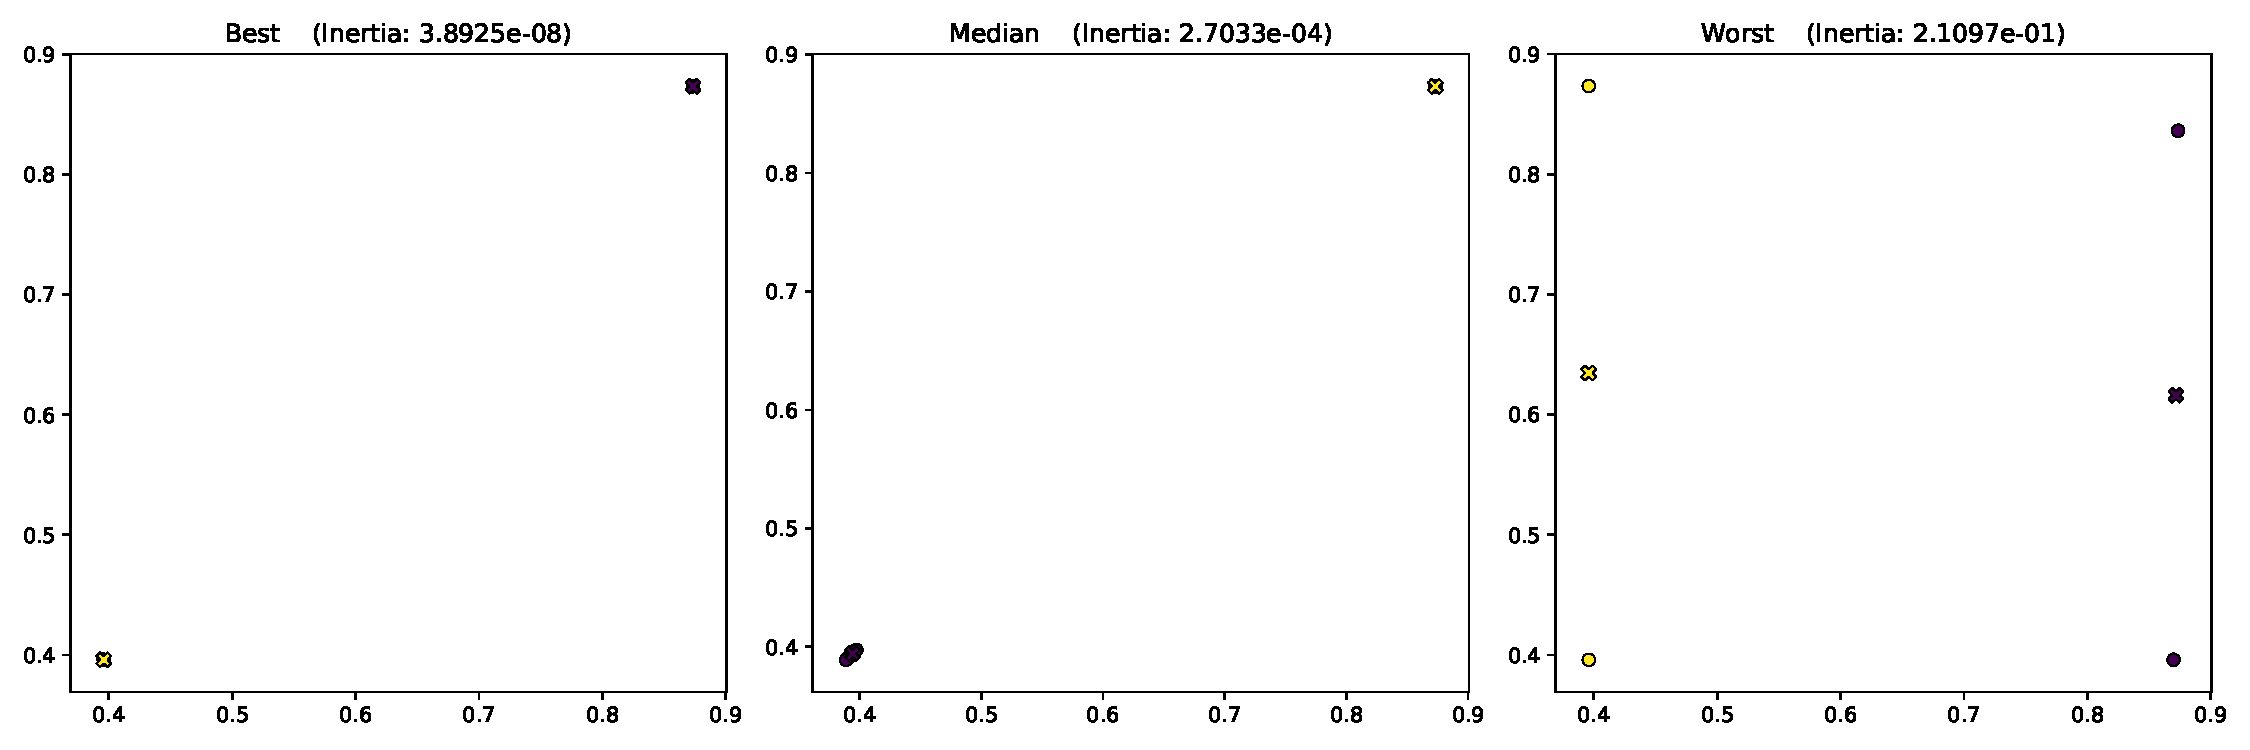
\includegraphics[width=\linewidth]{Fig10a.pdf}%
        \caption{}\label{fig:edo_variance}
    \end{subfigure}

    \begin{subfigure}{\imgwidth}
        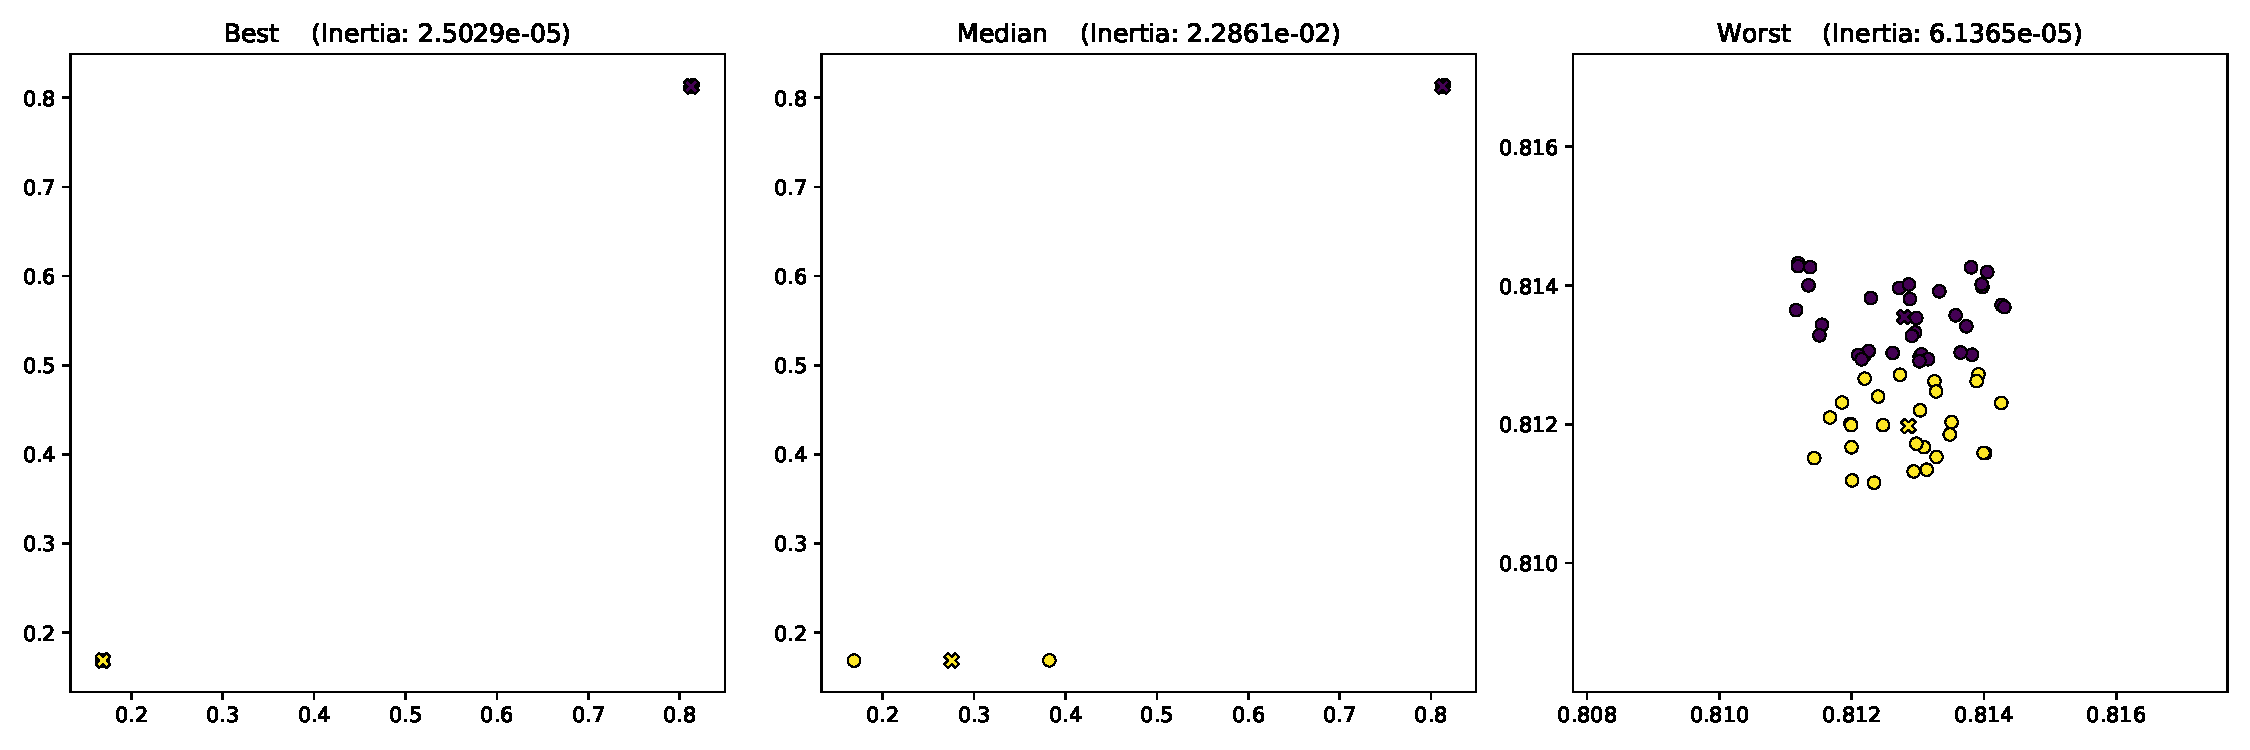
\includegraphics[width=\linewidth]{Fig10b.pdf}%
    \caption{}\label{fig:edo_skewness}
    \end{subfigure}

    \begin{subfigure}{\imgwidth}
        \includegraphics[width=\linewidth]{Fig10c.pdf}%
        \caption{}\label{fig:edo_kurtosis}
    \end{subfigure}
    \caption{Distribution plots for the (\subref{fig:edo_variance}) variance,
        (\subref{fig:edo_skewness}) skewness and (\subref{fig:edo_kurtosis})
        kurtosis of the first principal components in each
        case}\label{fig:edo_moments}
\end{figure}

\begin{figure}
    \centering
    \begin{subfigure}{\imgwidth}
        \includegraphics[width=\linewidth]{Fig11a.pdf}
        \caption{}\label{fig:edo_iqr}
    \end{subfigure}\vfill%

    \begin{subfigure}{\imgwidth}
        \includegraphics[width=\linewidth]{Fig11b.pdf}
        \caption{}\label{fig:edo_lower}
    \end{subfigure}\vfill%

    \begin{subfigure}{\imgwidth}
        \includegraphics[width=\linewidth]{Fig11c.pdf}
        \caption{}\label{fig:edo_upper}
    \end{subfigure}
    \caption{Distribution plots for the (\subref{fig:edo_iqr}) interquartile
        range, (\subref{fig:edo_lower}) lower decile and
        (\subref{fig:edo_upper}) upper decile of the first principal components
        in each case}\label{fig:edo_quantiles}
\end{figure}


\section{Chapter summary}\label{sec:kmodes:summary}

This chapter has introduced a novel initialisation method for the \(k\)-modes
algorithm that builds on the method set out in the seminal
paper~\cite{Huang1998}. The new method models the final replacement process in
the original as an instance of the hospital-resident assignment problem that may
be solved using a Gale-Shapley algorithm. The use of game theory here allows for
a more mathematically fair initialisation to \(k\)-modes, adding to the
literature around so-called `fair' machine learning.

Following a thorough description of the \(k\)-modes algorithm and the
established initialisation methods, a comparative analysis was conducted among
the three initialisations using benchmark datasets. In addition, the EDO method
described in Chapter~\ref{chp:edo} was utilised to extend this analysis to
artificial datasets.

The first of these analyses revealed that the proposed initialisation was able
to consistently outperform both of the other methods when the choice of \(k\)
had been optimised somewhat. However, the proposed method was unable to beat
Cao's method when an external, and frankly separate, framework was imposed on
each dataset by choosing \(k\) to be the number of classes present.

The latter analysis showed that the proposed method should be employed over
Cao's if there is no direct evidence that the dataset at hand has some notion of
high density. Otherwise, Cao's method remains the most reliable initialisation
in terms of computational time and final cost.
